\documentclass[a4paper]{article}
\usepackage[T1]{fontenc}
\usepackage{times,mathptm}
\usepackage[scaled=0.80]{beramono}
\usepackage{rascal}
\usepackage{highlight}
\usepackage{hyperref}
\usepackage{url}
\usepackage{epsfig}
\usepackage{float}

\def\source#1#2{\href{http://svn.rascal-mpl.org/lwc/trunk/lwc11/src/#1}{#2}}
\floatstyle{ruled}
\newfloat{listing}{htbp}{lol}
\floatname{listing}{Listing}

\begin{document}

\title{Language Workbench Comparison 2011 --- \Rascal}
\author{Tijs van der Storm\\
\textsl{CWI, Amsterdam}\\
\texttt{storm@cwi.nl}}
\maketitle

\section*{Introduction to \Rascal}

\begin{itemize}
\item Source-to-source
\item Modular syntax definition
\item Function programming language (immutable data)
\item IDE integration with Eclipse throug IMP
\end{itemize}

\section*{Phase 0}

\subsection*{Task 0.1: A Language for Entities}

\begin{listing}
\begin{rascal}
import lang::entities::syntax::Layout;
import lang::entities::syntax::Ident;
import lang::entities::syntax::Types;

start syntax Entities
    = entities: Entity* entities;

syntax Entity 
    = @Foldable entity: "entity" Name name "{" Field* "}";

syntax Field 
    = field: Type Ident name;
\end{rascal}
\caption{\source{lang/entities/syntax}{Syntax definition of
  entities.}}
\end{listing}

\begin{figure}
\begin{center}
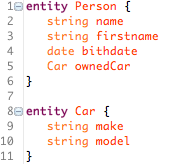
\epsfig{file=entities,width=0.3\linewidth}
\end{center}
\caption{Screenshot of an Eclipse editor showing highlighted entities\label{FIG:entities}}
\end{figure}

\begin{listing}
\begin{rascal}
data Entities = entities(list[Entity] entities);
    
data Entity = entity(Name name, list[Field] fields);
    
data Field = field(Type \type, str name);

data Type = primitive(PrimitiveType primitive)
          | reference(Name name);
    
data Name = name(str name);

data PrimitiveType = string() | date() | integer() | boolean();
\end{rascal}
\caption{\source{lang/entities/ast/Entities.rsc}{Abstract syntax of
    entities.}}
\end{listing}


\subsection*{Task 0.2: Code Generation To Java}

\begin{listing}
\begin{rascal}
public str entity2java(Entity e) {
    return "public class <e.name.name> {
        '<for (f <- e.fields) {>
        '  <field2java(f)>
        '<}>
        '}";
}

public str field2java(field(typ, n)) {
    <t, cn> = <type2java(typ), capitalize(n)>;
    return "private <t> <n>;
           'public <t> get<cn>() {
           '    return this.<n>;
           '}
           'public void set<cn>(<t> <n>) {
           '    this.<n> = <n>;
           '}";
}
\end{rascal}
\caption{\source{lang/entities/compile/Entities2Java.rsc}{Functions to
    generate Java classes.}}
\end{listing}

\subsection*{Task 0.3: Constraint Checking}

\begin{listing}
\begin{rascal}
public list[Message] check(Entities es) {
    defs = {};
    errors = for (e <- es.entities) {
        if (e.name in defs) {
            append error("Redeclared entity", e@location);
        }
        defs += {e.name};
    }
    return ( errors | it + checkEntity(e, defs) | e <- es.entities );
}

public list[Message] checkEntity(Entity e, set[Name] defs) {
    fs = {};
    return for (f <- e.fields) {
        if (f.name in fs) {
            append error("Duplicate field", f@location);
        }
        if (reference(Name n) := f.\type, n notin defs) {
            append error("Undefined entity type", n@location);
        }
        fs += {f.name};
    }
}
\end{rascal}
\caption{\source{lang/entities/check/Entities.rsc}{Functions to check
    entities for errors.}}
\end{listing}

\subsection*{Task 0.4: Breaking Down Models}

\begin{listing}
\begin{rascal}
public Entities merge(loc files...) {
    return merge({ parse(f) | f <- files });
}

public Entities merge(set[Entities] ess) {
    return entities(( [] | it + es.entities | es <- ess ));
}
\end{rascal}
\caption{\source{lang/entities/utils/Merge.rsc}{Utility functions to
    merge multiple entity files into a single set of entities}}
\end{listing}



\section{Phase 1}



\end{document}